\documentclass[11pt,a4paper]{article}

\usepackage[T1]{fontenc}
\usepackage[utf8]{inputenc}
\usepackage[french]{babel}
\usepackage{geometry}
\usepackage{graphicx}
\usepackage{booktabs}
\usepackage{tabularx}
\usepackage{float}
\usepackage{hyperref}
\usepackage{fancyhdr}
\usepackage{etoolbox}
\usepackage{needspace}
\preto{\section}{\Needspace{0.35\textheight}}
\preto{\subsection}{\Needspace{0.25\textheight}}
\preto{\subsubsection}{\Needspace{0.12\textheight}}

\geometry{margin=2.5cm}
\graphicspath{{images/}}
\setlength{\parindent}{0pt}
\setlength{\parskip}{0.5em}

\pagestyle{fancy}
\setlength{\headheight}{14pt}
\fancyhf{}
\lhead{Pangol1 -- Manuel d'Utilisation}
\rhead{\leftmark}
\cfoot{\thepage}

\hypersetup{
  colorlinks=true,
  linkcolor=black,
  urlcolor=black,
  citecolor=black,
  pdfauthor={Equipe Pangol1},
  pdftitle={Manuel d'Utilisation - Pangol1}
}

\begin{document}

\begin{titlepage}
  \centering
  \includegraphics[width=2cm]{logo.png}\\[1cm]
  {\Huge\bfseries Manuel d'Utilisation - Pangol1\par}
  \vfill
  {\large Version 1.0\\ \today\par}
\end{titlepage}

\tableofcontents
\listoffigures
\newpage

\section{Pangol1}
\emph{Guide complet : importation, analyse, visualisation et exportation}

\textbf{Pangol1} est une solution logicielle open source de haute performance sp\'ecialis\'ee la cr\'eation de rapports d'analyse de donn\'ees sur de tr\`es gros volumes de donn\'ees.

\subsection*{Table des mati\`eres}
\begin{enumerate}
  \item Interface du logiciel
  \item Configuration de l'application
  \item Tableau de donn\'ees
  \item Carnet de notes et exportation
  \item Support technique
\end{enumerate}

\section{Interface du logiciel}
\begin{figure}[H]
  \centering
  \includegraphics[width=0.6\linewidth]{main_view.png}
  \caption{Interface du logiciel}
\end{figure}

Voici la vue principale de \textbf{Pangol1}. Elle se compose de plusieurs sections cl\'es:

\begin{itemize}
  \item \textbf{Barre de menu} : Acc\`es aux fonctionnalit\'es principales (Fichier, Affichage, Aide).
  \newline Elle se situe en haut de l'interface et permet d'acc\'eder \`a toutes les fonctionnalit\'es du logiciel.
  \item \textbf{Barre d'information} : Affiche des informations sur les donn\'ees import\'ees et les analyses en cours.
  \newline Elle se trouve tout en bas de l'interface et fournit des informations contextuelles sur les donn\'ees et les analyses.
  \item \textbf{Carnet de notes} : Permet de cr\'e\'e de graphiques, ajouter des commentaires et m\^eme ajouter des images pour enrichir les rapports d'analyse.
  \newline Il est situ\'e \`a gauche de l'interface et offre un espace pour documenter les analyses et les r\'esultats.
  \item \textbf{Tableau de donn\'ees} : Affiche les donn\'ees cellule par cellule, permettant une manipulation directe.
  \newline Il est situ\'e sur la partie droite de l'interface.
\end{itemize}

\subsection{Barre de menu}
\subsubsection*{Menu Fichier}
Le menu ``Fichier'' permet d'ouvrir de nouvelles tables de donn\'ees, ou des tables r\'ecemment ouvertes ou encore d'acc\'eder aux param\`etres de configuration de l'application.

\begin{figure}[H]
  \centering
  \includegraphics[width=0.8\linewidth]{topbar_menu_file.png}
  \caption{Menu Fichier}
\end{figure}

\subsubsection*{Menu Affichage}
Le menu ``Affichage'' permet de personnaliser la disposition des \`elements de l'interface, d'afficher ou de masquer le carnet de notes, la table de donn\'ees, etc.

\begin{figure}[H]
  \centering
  \includegraphics[width=0.8\linewidth]{topbar_menu_display_panes.png}
  \caption{Menu Affichage - Panes}
\end{figure}

Il permet aussi de changer l'ordre des panneaux:

\begin{figure}[H]
  \centering
  \includegraphics[width=0.8\linewidth]{topbar_display_rotate.png}
  \caption{Menu Affichage - Rotation des panneaux}
\end{figure}

Et voici les une des dispositions possibles de l'interface:

\begin{figure}[H]
  \centering
  \includegraphics[width=0.8\linewidth]{main_display_rotate.png}
  \caption{Interface avec une disposition diff\'erente}
\end{figure}

\subsubsection*{Menu Aide}
Le menu ``Aide'' permet d'acc\'eder \`a la documentation, de voir les informations sur la version du logiciel et aussi de changer rapidement la langue de l'interface:

\begin{figure}[H]
  \centering
  \includegraphics[width=0.8\linewidth]{topbar_menu_help.png}
  \caption{Menu Aide}
\end{figure}

Information sur le logiciel:

\begin{figure}[H]
  \centering
  \includegraphics[width=0.8\linewidth]{main_about.png}
  \caption{Informations sur le logiciel}
\end{figure}

\subsection{Barre d'information}
La barre d'information permet d'afficher le statut de l'application et les t\^aches en cours:

\begin{figure}[H]
  \centering
  \includegraphics[width=0.8\linewidth]{bottombar_status.png}
  \caption{Barre d'information - Statut de l'application}
\end{figure}

Vous pouvez cliquer sur la barre de chargement pour afficher les d\'etails de la t\^ache en cours:

\begin{figure}[H]
  \centering
  \includegraphics[width=0.8\linewidth]{bottombar_task.png}
  \caption{Barre d'information - T\^ache en cours}
\end{figure}

Ici on observe que l'application est en cours de chargement d'une table qui proviens d'une URL:

\begin{figure}[H]
  \centering
  \includegraphics[width=0.8\linewidth]{bottombar_task_open.png}
  \caption{Barre d'information - T\^ache en cours}
\end{figure}

\section{Configuration de l'application}
L'application propose plusieurs options de configuration pour personnaliser l'exp\'erience utilisateur et optimiser les performances. Vous pouvez acc\'eder aux param\`etres de configuration en cliquant sur le menu ``Fichier'' dans la barre de menu, puis en s\'electionnant ``Param\`etres''.

\begin{figure}[H]
  \centering
  \includegraphics[width=0.8\linewidth]{topbar_menu_file.png}
  \caption{Menu Fichier}
\end{figure}

\subsection{Param\`etres g\'en\'eraux}
Voici le r\'esum\'e des options disponibles dans les param\`etres g\'en\'eraux :

\begin{itemize}
  \item \textbf{Langue} : Permet de choisir la langue de l'interface utilisateur.
  \item \textbf{D\'emarrage} : Configuration du comportement de l'application au d\'emarrage (ouvrir le dernier projet, afficher un \`ecran de bienvenue, etc.).
  \item \textbf{Fermeture} : Options pour la fermeture de l'application (confirmation avant de quitter, etc.).
\end{itemize}

\begin{figure}[H]
  \centering
  \includegraphics[width=0.8\linewidth]{settings_general.png}
  \caption{Param\`etres g\'en\'eraux}
\end{figure}

\subsubsection*{Langue}
Vous pouvez s\'el\'eectionner la langue de l'interface utilisateur parmi les options disponibles:

\begin{itemize}
  \item AR: Arabe
  \item EN: Anglais
  \item FR: Fran\c{c}ais
  \item ES: Espagnol
  \item ID: Indon\'esien
  \item PT: Portugais
  \item RU: Russe
  \item ZH: Chinois
  \item JA: Japonais
  \item TR: Turc
\end{itemize}

\subsubsection*{D\'emarrage}
Vous pouvez configurer le comportement de l'application au d\'emarrage :

\begin{itemize}
  \item Affichez ou non l'\'ecran de chargement de Pangol1.
  \item V\'erifiez les mises \`a jour au d\'emarrage de l'application.
  \item R\'eouvrir les dernier tableaux de donn\'ees.
  \item Ouvrir ou non un tableau de donn\'ees par d\'efaut:
  \begin{itemize}
    \item Depuis un fichier
    \item Depuis une URL
  \end{itemize}
\end{itemize}

\subsubsection*{Fermeture}
Vous pouvez configurer les options de fermeture de l'application :

\begin{itemize}
  \item Confirmer avant de quitter l'application.
  \item Confirmer avant de fermer un tableau de donn\'ees.
\end{itemize}

\subsection{Param\`etres du tableau de donn\'ees}
Voici le r\'esum\'e des options disponibles dans les param\`etres du tableau de donn\'ees :

\begin{itemize}
  \item \textbf{Mode} : Permet d'editer les donn\'ees directement dans le fichier source.
  \item \textbf{Affichage} : Configuration de l'affichage du tableau de donn\'ees.
  \item \textbf{Colonnes} : Options pour la gestion des colonnes (ajout, suppression, r\'eorganisation).
  \item \textbf{Statistiques} : Param\`etres pour les calculs statistiques appliqu\'es aux donn\'ees.
\end{itemize}

\begin{figure}[H]
  \centering
  \includegraphics[width=0.8\linewidth]{settings_table.png}
  \caption{Param\`etres du tableau de donn\'ees}
\end{figure}

\subsubsection*{Mode}
\begin{itemize}
  \item Ouvrir les donn\'ees en mode lecture seule ou en mode \`edition.
  \newline Le mode \`edition permet d'\'ecrire directement dans les cellules de la table.
  \item Autoriser la saisie manuelle de type
  \newline Le fichier source est typ\'e se qui signifie que les donn\'ees sont automatiquement converties dans le type de donn\'ees appropri\'e (num\'erique, texte, date, etc.). En activant cette option, vous pouvez saisir manuellement des donn\'ees dans les cellules sans que le logiciel tente de les convertir automatiquement.
  \newline Attention, cela peut entra\^iner des pertes de donn\'ees ou des erreurs d'analyse si les donn\'ees saisies ne sont pas conformes au type attendu.
  \item Sensibilit\'e \`a la convertion de type
  \newline Lorsque que la table n'est pas typ\'e \textbf{Pangol1} tente de d\'eviner le type de donn\'ees et si un type est anb\"igu, il
  \newline prend le type le plus pr\'esent dans la colonne. Par d\'efault cette option est r\'egl\'ee sur 95\%, ce qui signifie que si 95\% des donn\'ees d'une colonne sont de type num\'erique, la colonne sera consid\'er\'ee comme num\'erique et donc que le reste des donn\'ees (par exemple des cha\^ines de caract\`eres) seront converties en num\'erique (par exemple en NaN). En ajustant ce seuil, vous pouvez contr\^oler la rigueur avec laquelle le logiciel d\'etermine le type de donn\'ees d'une colonne.
\end{itemize}

\subsubsection*{Affichage}
\begin{itemize}
  \item Afficher ou masquer les num\'eros de ligne.
  \item Afficher les valeurs nulles
  \newline L'affichage des valeurs nulles peut \^etre utile pour identifier les donn\'ees manquantes ou les erreurs dans le jeu de donn\'ees. Cependant, cela peut \`egalement rendre le tableau plus difficile \`a lire si de nombreuses valeurs nulles sont pr\'esentes. En activant cette option, vous pouvez choisir d'afficher ou de masquer les valeurs nulles dans le tableau de donn\'ees. Attention, cette option peut impacter les performances.
\end{itemize}

\subsubsection*{Colonnes}
\begin{itemize}
  \item Masquer les colonnes vides par d\'efaut
  \newline Lorsque cette option est activ\'ee, les colonnes qui ne contiennent aucune donn\'ee (c'est-\`a-dire des colonnes enti\`erement vides) seront automatiquement masqu\'ees dans le tableau de donn\'ees. Cela peut aider \`a r\'eduire l'encombrement visuel et \`a se concentrer sur les donn\'ees pertinentes. Cependant, si vous avez besoin de voir toutes les colonnes, y compris celles qui sont vides, vous pouvez d\'esactiver cette option.
  \item Afficher les types de donn\'ees dans les en-t\^etes de colonnes
  \newline En activant cette option, les types de donn\'ees (par exemple, num\'erique, texte, date) seront affich\'es dans les en-t\^etes de colonnes du tableau de donn\'ees. Cela peut \^etre utile pour identifier rapidement le type de donn\'ees contenu dans chaque colonne, ce qui peut faciliter l'analyse et la manipulation des donn\'ees.
  \item Ajuster automatiquement la largeur des colonnes
  \newline Lorsque cette option est activ\'ee, la largeur des colonnes du tableau de donn\'ees sera automatiquement ajust\'ee en fonction du contenu de chaque colonne. Cela signifie que les colonnes s'\'elargiront ou se r\'etr\'eciront pour s'adapter au texte ou aux valeurs qu'elles contiennent, ce qui peut am\'eliorer la lisibilit\'e du tableau.
\end{itemize}

\subsubsection*{Statistiques}
\begin{itemize}
  \item Calculer les statistiques lorsqu'une colonne est s\'electionn\'ee
  \newline En activant cette option, les statistiques de base (telles que la moyenne, la m\'ediane, l'\'ecart-type, etc.) seront automatiquement calcul\'ees et affich\'ees lorsque vous s\'electionnez une colonne dans le tableau de donn\'ees. Cela peut \^etre utile pour obtenir rapidement des informations sur la distribution des donn\'ees dans cette colonne sans avoir \`a effectuer des calculs manuels. Attention, cette option peut impacter les performances.
\end{itemize}

\subsection{Param\`etres d'apparance}
Voici les r\'esum\'e des options disponibles dans les param\`etres d'apparance :

\begin{itemize}
  \item \textbf{Th\`eme} : Choix entre diff\'erents th\`emes d'apparence pour l'interface utilisateur (clair, sombre, etc.).
  \item \textbf{Interface} : Configuration de l'interface utilisateur (taille des polices, couleurs, etc.).
\end{itemize}

\begin{figure}[H]
  \centering
  \includegraphics[width=0.8\linewidth]{settings_appearance.png}
  \caption{Param\`etres du tableau de donn\'ees}
\end{figure}

\subsubsection*{Th\`eme}
\begin{itemize}
  \item Choix entre le th\`eme clair et le th\`eme sombre.
  \newline Le mode ``Automatique'' permet de choisir avec les curseurs votre plage horaire de pr\'ef\'erence pour le th\`eme sombre. Par d\'efaut, le th\`eme sombre est activ\'e de 18h \`a 6h du matin.
  \newline Le mode ``Syst\`eme'' permet d'adapter automatiquement le th\`eme de l'application en fonction du th\`eme de votre syst\`eme d'exploitation.
\end{itemize}

\subsubsection*{Interface}
\begin{itemize}
  \item Utiliser le th\`eme FlatLaf
  \newline FlatLaf est un th\`eme d'apparence moderne et \`epur\'e pour les applications Java. En activant cette option, vous pouvez appliquer le th\`eme FlatLaf \`a l'interface de Pangol1, ce qui peut am\'eliorer l'esth\'etique et la convivialit\'e de l'application. Attention, cette option peut impacter les performances sur les machines plus anciennes ou moins puissantes.
  \item Taille de la police
  \newline Vous pouvez ajuster la taille de la police utilis\'ee dans l'interface de Pangol1 pour am\'eliorer la lisibilit\'e en fonction de vos pr\'ef\'erences.
  \item Famille de police
  \newline Vous pouvez choisir la famille de police utilis\'ee dans l'interface de Pangol1 pour personnaliser l'apparence du texte selon vos pr\'ef\'erences. La liste des familles d\'epend exclusivement de celles install\'ees sur votre syst\`eme.
\end{itemize}

\subsection{Raccourcis clavier}
Pangol1 ne permet pas encore de personnaliser les raccourcis clavier, mais voici la liste des raccourcis disponibles par d\'efaut :

\begin{center}
\begin{tabularx}{0.9\linewidth}{@{}lX@{}}
\toprule
Action & Raccourci clavier \\
\midrule
Ouvrir une table & Ctrl + O \\
Fermer la table & Ctrl + W \\
Ouvrir le cr\'eateur de filtres & Ctrl + F \\
Ouvrir les param\`etres & Ctrl + , \\
Trie par ordre croissant & Ctrl + Shift + A \\
Trie par ordre d\'ecroissant & Ctrl + Shift + D \\
Annuler une action dans le carnet de notes & Ctrl + Z \\
R\'etablir une action dans le carnet de notes & Ctrl + Y \\
\bottomrule
\end{tabularx}
\end{center}

\begin{figure}[H]
  \centering
  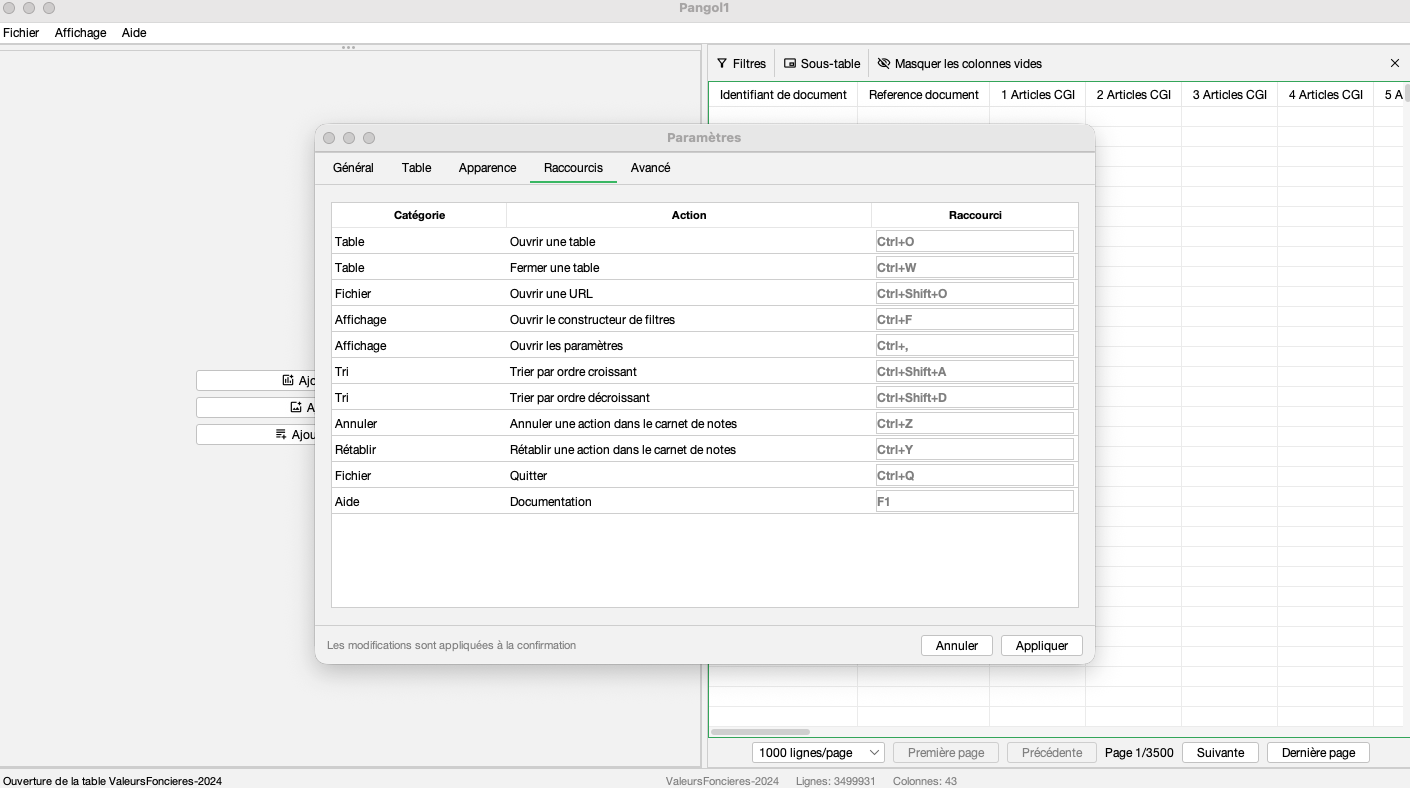
\includegraphics[width=0.8\linewidth]{settings_shortcuts.png}
  \caption{Param\`etres des raccourcis clavier}
\end{figure}

\subsection{Param\`etres avanc\'es}
Les param\`etres avanc\'es permettent de configurer des options plus techniques et sp\'ecifiques pour les utilisateurs exp\'eriment\'es. Voici un r\'esum\'e des options disponibles dans les param\`etres avanc\'es :

\begin{itemize}
  \item \textbf{Activer le journal de d\'ebogage} : Permet d'activer ou de d\'esactiver le journal de d\'ebogage pour aider \`a diagnostiquer les probl\`emes.
  \item \textbf{Activer le mode d\'eveloppeur} : Permet d'acc\'eder \`a des fonctionnalit\'es suppl\'ementaires destin\'ees aux d\'eveloppeurs.
\end{itemize}

\begin{figure}[H]
  \centering
  \includegraphics[width=0.8\linewidth]{settings_advanced.png}
  \caption{Param\`etres avanc\'es}
\end{figure}

\section{Tableau de donn\'ees}
Le panneau de droite de l'interface affiche les donn\'ees import\'ees dans un format de tableau. Chaque cellule du tableau correspond \`a une valeur sp\'ecifique dans le jeu de donn\'ees, et les utilisateurs peuvent interagir directement avec ces cellules pour manipuler les donn\'ees.
Ce panneau contient plusieur fonctionnalit\'es pour faciliter la manipulation et l'analyse des donn\'ees, notamment :

\begin{itemize}
  \item \textbf{Barre d'outils de la table} : Permet d'acc\'eder \`a des fonctionnalit\'es sp\'ecifiques pour manipuler les donn\'ees du tableau, telles que le tri, le filtrage, l'ajout ou la suppression de colonnes, etc.
  \item \textbf{Menu contextuel} : En cliquant avec le bouton droit sur l'en-t\^ete d'une colonne.
  \item \textbf{S\'election de colonnes} : Permet de s\'el\'ectionner une colonne et d'afficher ses statisitques de base (moyenne, m\'ediane, \`ecart-type, etc.) dans la barre d'information en bas de l'interface.
\end{itemize}

\subsection{Barre d'outils de la table}
La barre d'outils contient 4 boutons principaux pour manipuler les donn\'ees du tableau :

\begin{itemize}
  \item \textbf{Filtres} : Permet d'ouvrir le cr\'eateur de filtres pour appliquer des filtres avanc\'es sur les donn\'ees du tableau.
  \item \textbf{Sous-table} : Permet de cr\'eer une sous-table \`a partir des donn\'ees s\'electionn\'ees dans le tableau.
  \item \textbf{Afficher/Masquer les colonnes vides} : Permet d'afficher ou de masquer les colonnes qui ne contiennent aucune donn\'ee.
  \item \textbf{Fermer la table} : Permet de fermer le tableau de donn\'ees actuellement ouvert.
\end{itemize}

\subsubsection*{Cr\'eateur de filtres}
Le cr\'eateur de filtres permet d'appliquer des filtres avanc\'es sur le tableau ouvert. Vous pouvez cr\'eer des filtres bas\'es sur des conditions sp\'ecifiques pour affiner les donn\'ees affich\'ees dans le tableau. Par exemple, vous pouvez filtrer les donn\'ees pour n'afficher que les lignes o\`u une certaine colonne contient une valeur sp\'ecifique, ou pour n'afficher que les lignes o\`u une colonne num\'erique est sup\'erieure \`a un certain seuil.

\begin{figure}[H]
  \centering
  \includegraphics[width=0.8\linewidth]{table_toolbar_filter.png}
  \caption{Cr\'eateur de filtres}
\end{figure}

Voici un exemple de filtrage avanc\'e sur les donn\'ees du tableau:

\begin{figure}[H]
  \centering
  \includegraphics[width=0.8\linewidth]{filter_all.png}
  \caption{Exemple de filtrage avanc\'e}
\end{figure}

S\'election du filtre \`a appliquer, par exemple entre une \textbf{Intervale}:

\begin{figure}[H]
  \centering
  \includegraphics[width=0.8\linewidth]{filter_choose.png}
  \caption{Exemple de filtrage avanc\'e}
\end{figure}

Comme les colonnes sont typ\'ees le cr\'eateur de filtres est intelligent et ne propose que des op\'erateurs et des champs pertinent en fonction du type de la colonne s\'electionn\'ee.

Par exemple pour une colonne de type Date:

\begin{figure}[H]
  \centering
  \includegraphics[width=0.8\linewidth]{filter_date.png}
  \caption{Cr\'eateur de filtres pour une colonne de type Date}
\end{figure}

Pour une colonne de type Num\'erique:

\begin{figure}[H]
  \centering
  \includegraphics[width=0.8\linewidth]{filter_number.png}
  \caption{Cr\'eateur de filtres pour une colonne de type Num\'erique}
\end{figure}

Pour une colonne qui contient des cha\^ines de caract\`eres (ou une \textbf{Cat\'egorie}):

\begin{figure}[H]
  \centering
  \includegraphics[width=0.8\linewidth]{filter_category.png}
  \caption{Cr\'eateur de filtres pour une colonne de type Cha\^ine de caract\`eres}
\end{figure}

Les cat\'egorie dans \textbf{Pangol1} sont des colonnes de type cha\^ine de caract\`eres qui contiennent un nombre limit\'e de valeurs uniques. Par exemple, une colonne ``Pays'' qui contient les valeurs ``France'', ``Espagne'', ``Italie'', etc. Les cat\'egories sont trait\'ees de mani\`ere sp\'eciale dans le cr\'eateur de filtres pour permettre des filtrages plus efficaces et pertinents.

\subsubsection*{Sous-table}
Le concept de sous-table permet de cr\'eer une nouvelle table sur la base de la table ouverte. Il suffit de s\'electionner la colonne \`a partir de laquelle vous souhaitez regrouper les donn\'ees puis des choisir l'aggr\'egation de votre choix sur le reste des colonnes.

\begin{figure}[H]
  \centering
  \includegraphics[width=0.8\linewidth]{table_toolbar_subtable.png}
  \caption{Cr\'eateur de sous-table}
\end{figure}

Ici on s\'electionne une colonne qui contient des cat\'egories. Les colonnes sans aggr\'egation \textbf{(Aucune)} sont simplement ignor\'ees lors de la cr\'eation de la sous-table. Ici on choisit l'aggr\'egation de comptage distinct des \`elements:

\begin{figure}[H]
  \centering
  \includegraphics[width=0.8\linewidth]{subtable_create.png}
  \caption{Cr\'eateur de sous-table}
\end{figure}

Ensuite notre sous-table s'affiche comme un nouvelle table classique et elle est automatiquement sauvegard\'ee dans le m\^eme dossier que la table d'origine:

\begin{figure}[H]
  \centering
  \includegraphics[width=0.8\linewidth]{subtable_newtable.png}
  \caption{Sous-table cr\'e\'ee}
\end{figure}

\subsubsection*{Afficher/Masquer les colonnes vides}
Si votre table contient de nombreuses colonnes vides, cela peut rendre la navigation et l'analyse des donn\'ees plus difficile. En activant cette option, vous pouvez choisir d'afficher toutes les colonnes ou bien de masquer les colonnes qui ne contiennent aucune donn\'ee.

\begin{figure}[H]
  \centering
  \includegraphics[width=0.8\linewidth]{table_toolbar_hide_empty.png}
  \caption{Afficher/Masquer les colonnes vides}
\end{figure}

\subsubsection*{Fermer la table}
Lorque vous souhaitez change de table ou simplement fermer la table de donn\'ees. Vous pouvez revenir \`a la liste de vos tables ouvertes:

\begin{figure}[H]
  \centering
  \includegraphics[width=0.8\linewidth]{table_close.png}
  \caption{Fermer la table}
\end{figure}

Liste des tables ouvertes:

\begin{figure}[H]
  \centering
  \includegraphics[width=0.8\linewidth]{table_list_menu.png}
  \caption{Liste des tables ouvertes}
\end{figure}

Vous trouverez \`egalement un petit menu contextuel en cliquant avec le bouton droit sur une table de la liste.

\subsection{Menu contextuel}
En cliquant avec le bouton droit sur l'en-t\^ete d'une colonne, vous pouvez acc\'eder \`a un menu contextuel qui offre plusieurs options pour manipuler les donn\'ees de cette colonne. Voici les options disponibles dans le menu contextuel :

\begin{figure}[H]
  \centering
  \includegraphics[width=0.8\linewidth]{table_ctxmenu.png}
  \caption{Menu contextuel de la table}
\end{figure}

\begin{itemize}
  \item \textbf{Trier} : Permet de trier les donn\'ees de la colonne par ordre croissant ou d\'ecroissant.
  \item \textbf{Appliquer un filtre simple} : Permet d'appliquer un filtre simple sur la colonne, en s\'electionnant une valeur sp\'ecifique \`a afficher.
  \item \textbf{Afficher les statistiques} : Permet d'afficher les statistiques de base pour la colonne s\'electionn\'ee, telles que la moyenne, la m\'ediane, l'\'ecart-type, etc.
  \item \textbf{Changer le type de donn\'ees} : Permet de changer le type de donn\'ees de la colonne (num\'erique, texte, date, etc.).
  \item \textbf{Renommer la colonne} : Permet de renommer la colonne pour une meilleure organisation des donn\'ees.
  \item \textbf{Masquer la colonne} : Permet de masquer la colonne du tableau de donn\'ees.
\end{itemize}

\subsubsection*{Trie par ordre croissant ou d\'ecroissant}
Attention si le trie est appliqu\'e sur plusieurs colonnes, le trie ne sera effectif uniquement sur la derni\`ere colonne sur laquelle le trie a \'et\'e appliqu\'e. Par exemple, si vous appliquez un trie croissant sur la colonne ``Pays'' puis un trie d\'ecroissant sur la colonne ``Population'', les donn\'ees seront tri\'ees par ordre d\'ecroissant de population, et en cas d'\'egalit\'e de population, elles seront tri\'ees par ordre croissant de pays.

\begin{figure}[H]
  \centering
  \includegraphics[width=0.8\linewidth]{table_ctxmenu_sort.png}
  \caption{Trier les donn\'ees de la colonne}
\end{figure}

\subsubsection*{Appliquer un filtre simple}
Le filtre simple permet de filtrer les donn\'ees uniquement sur une colonne. Ce menu contextuel est intelligent et s'adapte au type de donn\'ees de la colonne s\'electionn\'ee. Par exemple, pour une colonne de type cat\'egorie, le menu contextuel affichera la liste des cat\'egories uniques pr\'esentes dans la colonne, et vous pourrez s\'electionner une ou plusieurs cat\'egories pour filtrer les donn\'ees.

\begin{figure}[H]
  \centering
  \includegraphics[width=0.8\linewidth]{table_ctxmenu_filter.png}
  \caption{Appliquer un filtre simple}
\end{figure}

Ici on applique un filtre par \textbf{Cat\'egorie} sur une colonne qui a \'et\'e d\'etect\'ee comme contenant des cat\'egories. Le menu contextuel affiche la liste des cat\'egories uniques pr\'esentes dans la colonne, et vous pouvez s\'electionner une ou plusieurs cat\'egories pour filtrer les donn\'ees.

\begin{figure}[H]
  \centering
  \includegraphics[width=0.8\linewidth]{table_ctxmenu_filter_category.png}
  \caption{Appliquer un filtre simple sur une colonne de type cat\'egorie}
\end{figure}

Le boutton ``Supprimer les filtres'' permet de supprimer tous les filtres appliqu\'es sur la \textbf{colonne} s\'electionn\'ee et non sur l'ensemble du tableau.

\subsubsection*{Afficher les statistiques}
Le menu de statistiques est lui aussi intelligent et s'adapte en fonction du type de donn\'ees de la colonne s\'electionn\'ee.

\begin{figure}[H]
  \centering
  \includegraphics[width=0.8\linewidth]{table_ctxmenu_stats.png}
  \caption{Afficher les statistiques de la colonne}
\end{figure}

Par exemple pour le type date:

\begin{figure}[H]
  \centering
  \includegraphics[width=0.8\linewidth]{table_ctxmenu_stats_date.png}
  \caption{Afficher les statistiques pour une colonne de type date}
\end{figure}

Pour le type num\'erique les options sont bien plus nombreuses:

\begin{figure}[H]
  \centering
  \includegraphics[width=0.8\linewidth]{table_ctxmenu_stats_number.png}
  \caption{Afficher les statistiques pour une colonne de type num\'erique}
\end{figure}

Vous remarquerez qu'il existe des options de corr\'elations pour les colonnes num\'eriques. Cette option permet de calculer la corr\'elation entre la colonne s\'electionn\'ee et une autre colonne num\'erique de votre choix.

Lorsque vous s\'electionnez par exemple l'option \textbf{R\'esumer}, une nouvelle fen\^etre s'ouvre pour vous permettre de visualiser les statistiques.

\begin{figure}[H]
  \centering
  \includegraphics[width=0.8\linewidth]{stats_summary.png}
  \caption{R\'esum\'e des statistiques pour une colonne de type num\'erique}
\end{figure}

Vous pouvez ensuite les ajouter au carnet de notes en cliquant sur le bouton ``Ajouter au carnet de notes'' en bas de la fen\^etre.

\begin{figure}[H]
  \centering
  \includegraphics[width=0.8\linewidth]{stats_summary_add.png}
  \caption{Ajouter les statistiques au carnet de notes}
\end{figure}

\subsubsection*{Autres options du menu contextuel}
\begin{itemize}
  \item \textbf{Changer le type de donn\'ees} : Cette option n'est visible que pour les utilisateurs qui on activ\'e dans les param\`etres le mode \`edition: ``Table>Mode>Autoriser la saisie manuelle de type''. Elle permet de changer le type de donn\'ees d'une colonne, par exemple de num\'erique \`a texte ou de date \`a texte, etc. Attention, cela peut entra\^iner des pertes de donn\'ees ou des erreurs d'analyse si les donn\'ees ne sont pas conformes au type attendu.
  \item \textbf{Renommer la colonne} : Permet de renommer la colonne pour une meilleure organisation des donn\'ees. Par exemple, vous pouvez renommer une colonne ``Population'' en ``Population totale''. Attention, le renommage ne s'applique que visuellement dans le tableau de donn\'ees et n'affecte pas le nom de la colonne dans le fichier source.
  \item \textbf{Masquer la colonne} : Permet de masquer la colonne du tableau de donn\'ees.
\end{itemize}

\subsection{S\'el\'eection de colonnes}
Si vous avez activ\'e dans les param\`etres l'option ``Table>Statistiques>Calculer les statistiques lorsqu'une colonne est s\'electionn\'ee'', vous pouvez simplement cliquer sur une colonne du tableau de donn\'ees pour afficher ses statistiques de base (moyenne, m\'ediane, \`ecart-type, etc.) dans la barre d'information en bas de l'interface.

\begin{figure}[H]
  \centering
  \includegraphics[width=0.8\linewidth]{bottombar_stats.png}
  \caption{S\'election de colonnes et affichage des statistiques}
\end{figure}

\section{Carnet de notes et exportation}
Le carnet de notes vous permet de documenter votre analyse sur les donn\'ees en ajoutant des graphiques, des commentaires et m\^eme des images. Vous pouvez cr\'eer plusieurs pages dans le carnet de notes pour organiser votre analyse de mani\`ere structur\'ee.

Les blocs du carnet de notes sont d\'epla\c{c}ables et modifiables:

\begin{figure}[H]
  \centering
  \includegraphics[width=0.8\linewidth]{report_ctxmenu.png}
  \caption{Menu contextuel du carnet de notes}
\end{figure}

Vous pouvez \`egalement les d\'eplacer avec le ``glisser-d\'eposer'' pour organiser votre page comme vous le souhaitez:

\begin{figure}[H]
  \centering
  \includegraphics[width=0.8\linewidth]{report_dragdrop.png}
  \caption{Glisser-d\'eposer dans le carnet de notes}
\end{figure}

\subsubsection*{Ajouter un texte}
Cliquer sur le button ``Ajouter un bloc de texte'':

\begin{figure}[H]
  \centering
  \includegraphics[width=0.8\linewidth]{report_select_text.png}
  \caption{Ajouter un texte au carnet de notes}
\end{figure}

Puis saisissez votre texte dans la section de param\'etrage du bloc de texte:

\begin{figure}[H]
  \centering
  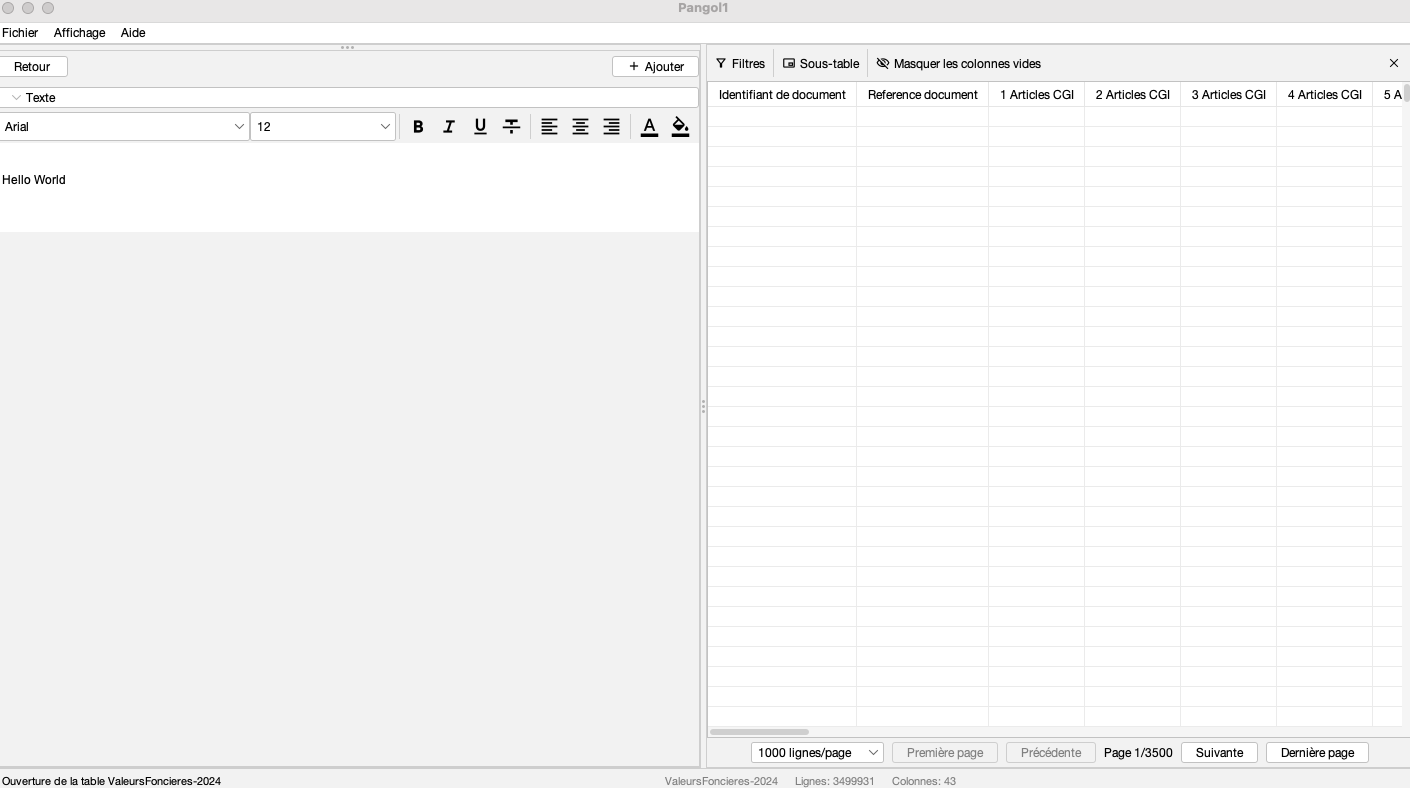
\includegraphics[width=0.8\linewidth]{report_text_setting.png}
  \caption{Param\`etres du bloc de texte}
\end{figure}

Et voici le r\'esultat dans le carnet de notes:

\begin{figure}[H]
  \centering
  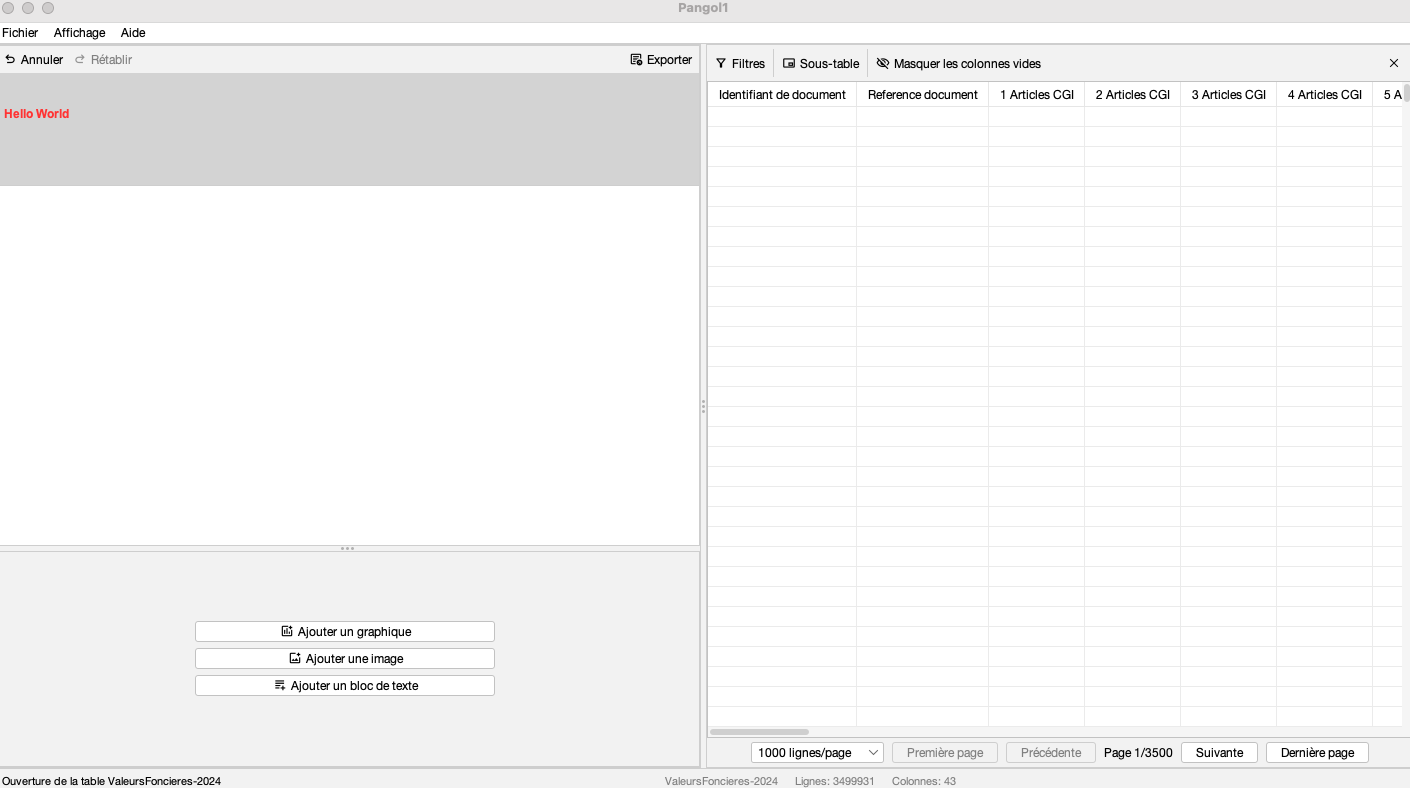
\includegraphics[width=0.8\linewidth]{report_text.png}
  \caption{Bloc de texte ajout\'e au carnet de notes}
\end{figure}

\subsubsection*{Ajouter une image}
Cliquer sur le button ``Ajouter une image'':

\begin{figure}[H]
  \centering
  \includegraphics[width=0.8\linewidth]{report_select_image.png}
  \caption{Ajouter une image au carnet de notes}
\end{figure}

Puis s\'electionnez votre image parmis vos fichiers:

\begin{figure}[H]
  \centering
  \includegraphics[width=0.8\linewidth]{report_image_setting.png}
  \caption{Param\`etres du bloc dimage}
\end{figure}

Et voici le r\'esultat dans le carnet de notes:

\begin{figure}[H]
  \centering
  \includegraphics[width=0.8\linewidth]{report_image.png}
  \caption{Image ajout\'ee au carnet de notes}
\end{figure}

\subsubsection*{Ajouter un graphique}
Cliquer sur le button ``Ajouter un graphique'':

\begin{figure}[H]
  \centering
  \includegraphics[width=0.8\linewidth]{report_select_chart.png}
  \caption{Ajouter un graphique au carnet de notes}
\end{figure}

Ensuite une menu de param\'etrage souvre et vous offre plusieurs sections pour configurer votre graphique:

\begin{figure}[H]
  \centering
  
\includegraphics[width=0.8\linewidth]{report_chart_setting.png}
  \caption{Param\`etres du bloc de graphique}
\end{figure}

Vous pouvez choisir la source de vos donn\'ees et m\^eme travailler sans avoir de table ouverte:

\begin{figure}[H]
  \centering
  \includegraphics[width=0.8\linewidth]{report_select_table.png}
  \caption{S\'election de la source de donn\'ees pour le graphique}
\end{figure}

Ensuite ajouter votre graphique dans le carnet de notes:

\begin{figure}[H]
  \centering
  \includegraphics[width=0.8\linewidth]{report_chart.png}
  \caption{Graphique ajout\'e au carnet de notes}
\end{figure}

Si vous aviez envie de modifier votre graphique, double-cliquez simplement dessus pour rouvrir le menu de param\'etrage qui cette fois ci contiendra des options suppl\'ementaires pour modifier votre graphique:

\begin{figure}[H]
  \centering
  \includegraphics[width=0.8\linewidth]{report_chart_edit.png}
  \caption{Modifier un graphique dans le carnet de notes}
\end{figure}

Une fois terminer cliquer simplement sur ``Modifier'' pour appliquer les modifications \`a votre graphique.
Voici les diff\'erents graphiques que \textbf{Pangol1} propose:

\begin{figure}[H]
  \centering
  \includegraphics[width=0.3\linewidth]{chart_bar.png}
  \includegraphics[width=0.3\linewidth]{chart_cols.png}
  \includegraphics[width=0.3\linewidth]{chart_line.png}
  \caption{Graphiques en barres, en colonnes et en lignes}
\end{figure}

\begin{figure}[H]
  \centering
  \includegraphics[width=0.3\linewidth]{chart_pie.png}
  \includegraphics[width=0.3\linewidth]{chart_radar.png}
  \includegraphics[width=0.3\linewidth]{chart_dots.png}
  \caption{Graphiques en camembert, en nuage de points et en radar}
\end{figure}

\begin{figure}[H]
  \centering
  \includegraphics[width=0.3\linewidth]{chart_area.png}
  \caption{Graphique en aires}
\end{figure}

Les graphiques disponibles incluent : graphique en barres, graphique en colonnes, graphique en lignes, graphique en camembert, graphique en nuage de points, graphique en radar, graphique en aires.

\subsection{Exporter le carnet de notes}
Une fois votre analyse termin\'ee, vous pouvez exporter votre carnet de notes dans plusieurs formats et diff\'erents styles:

\begin{figure}[H]
  \centering
  \includegraphics[width=0.8\linewidth]{report_export.png}
  \caption{Exporter le carnet de notes}
\end{figure}

\begin{figure}[H]
  \centering
  \includegraphics[width=0.8\linewidth]{export_main.png}
  \caption{Menu d'exportation du carnet de notes}
\end{figure}

S\'election du format d'exportation:

\begin{figure}[H]
  \centering
  \includegraphics[width=0.8\linewidth]{export_format.png}
  \caption{S\'election du format d'exportation}
\end{figure}

S\'election du style d'exportation:

\begin{figure}[H]
  \centering
  
\includegraphics[width=0.8\linewidth]{export_theme.png}
  \caption{S\'election du style d'exportation}
\end{figure}

Ensuite vous pourrez choisir le dossier de destination de votre rapport et trouver un fichier ZIP contenant:

\begin{itemize}
  \item Un fichier au format de votre choix (HTML, PDF, Markdown, etc.) avec votre rapport d'analyse.
  \item Un dossier ``charts'' contenant les images en SVG et en PNG de touts les graphiques que vous avez cr\'e\'es dans votre carnet de notes.
\end{itemize}

\section{Support Technique}
Pour tout probl\`eme :

\begin{itemize}
  \item \textbf{Jules Garcia} (Scrum Master)  \\
  \href{mailto:jules.garcia.1@etudiant.univ-rennes1.fr}{jules.garcia.1@etudiant.univ-rennes1.fr}
  \item \textbf{Kerem Eylem} (Product Owner)  \\
  \href{mailto:kerem.eylem@etudiant.univ-rennes1.fr}{kerem.eylem@etudiant.univ-rennes1.fr}
  \item \textbf{Briac Boitel} (Developer)  \\
  \href{mailto:briac.boitel@etudiant.univ-rennes.fr}{briac.boitel@etudiant.univ-rennes.fr}
  \item \textbf{No\'e Berthelier} (Developer)  \\
  \href{mailto:noe.berthelier@etudiant.univ-rennes1.fr}{noe.berthelier@etudiant.univ-rennes1.fr}
  \item \textbf{Elouan Barbier} (Developer)  \\
  \href{mailto:elouan.barbier.1@etudiant.univ-rennes1.fr}{elouan.barbier.1@etudiant.univ-rennes1.fr}
  \item \textbf{Paul Gallon} (Developer)  \\
  \href{mailto:paul.gallon@etudiant.univ-rennes.fr}{paul.gallon@etudiant.univ-rennes.fr}
  \item \textbf{Basile Guemene} (Developer)  \\
  \href{mailto:basile.guemene@etudiant.univ-rennes.fr}{basile.guemene@etudiant.univ-rennes.fr}
\end{itemize}

\end{document}
